% Intended LaTeX compiler: pdflatex
\documentclass[10pt,a4paper,UTF8]{article}
\usepackage{zclorg}
\author{emacsun}
\date{}
\title{维度诅咒}
\hypersetup{
 pdfauthor={emacsun},
 pdftitle={维度诅咒},
 pdfkeywords={},
 pdfsubject={},
 pdfcreator={Emacs 25.0.50.1 (Org mode 9.0.5)},
 pdflang={English}}
\begin{document}

\maketitle
\tableofcontents
\titlepic{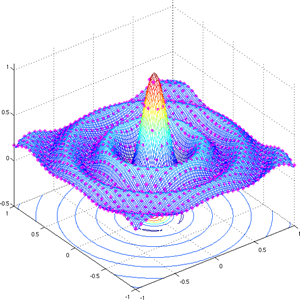
\includegraphics[scale=0.25]{../../img/sinc.PNG}}

\section{回忆}
\label{sec:org385ff7c}


在 \href{PRMLch1dot1-polynomial-curve.org}{多项式拟合} 问题中,输入的测试集\(x\)是一维的,估计的目标值\(t\)也是一维的。这个模型是模式识别中的 "toy" 模型,主要用来引入模式识别中的相关概念。在实际应用中,输入测试集往往是高维的,随着维度的提升,原先不是问题的地方也会有问题浮现。

\section{最近邻算法}
\label{sec:org20f43c4}


现在我们考虑一个分类问题,目标可以分三类。即,对于一个输入,输出是三个中的一个。为了简化问题,我们考虑输入是个二维向量\((x_{1},x_{2})\)。这么做仅仅是为了简化问题,并不代表所有输入都是这么低的维度。假设我们已经有了100个训练集,其分布如图\ref{fig:org87fdd7e}所示。蓝色绿色和红色分别代表不同的分类。
\begin{figure}[htbp]
\centering
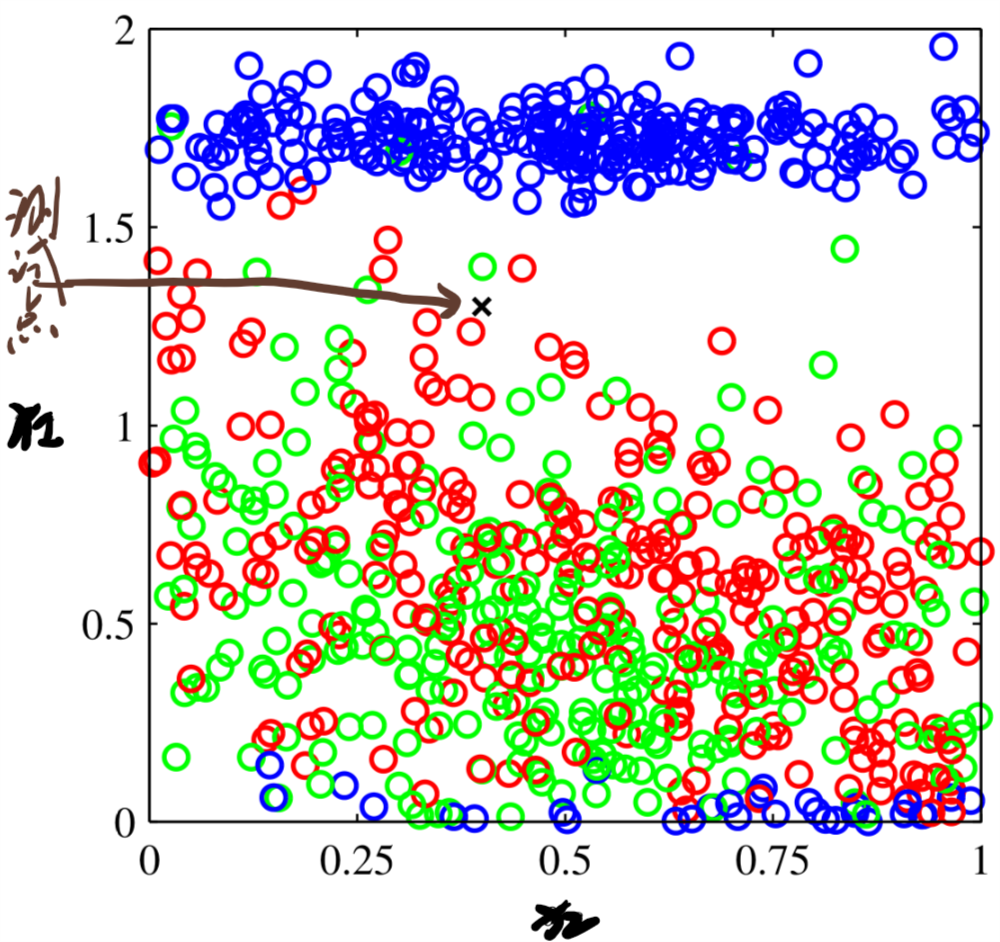
\includegraphics[width=0.6\textwidth]{../../img/computer_prml/20170503figure1dot19.png}
\caption{\label{fig:org87fdd7e}
二维输入的分类问题模型}
\end{figure}

对于输入(图\ref{fig:org87fdd7e} 中用黑色叉表示),我们要估计其属于黑色,蓝色或者绿色中的哪一类。一个最直观的输出是看看它周围的都是什么类型。如何把这个思想转化位算法?一个最简单的实现就是把输入空间划分成大小相等的胞元,如图\ref{fig:orgc0c41b0}所示。

通过对输入空间进行胞元划分,我们只需要统计新的输入落入的胞元中哪种类型占比最大就可以。这种方法叫做最近邻算法。这种简单粗暴的最近邻算法有很多的问题,但是最致命的一个就是当输入矢量维度变大时带来的复杂度问题,即维度诅咒。设想:我们现在的输入是二维向量,但是当输入是三维,四位甚至更高维呢?问题就变得复杂起来。因为输入的维度变高后,胞元的数量也成指数上升。
\begin{figure}[htbp]
\centering
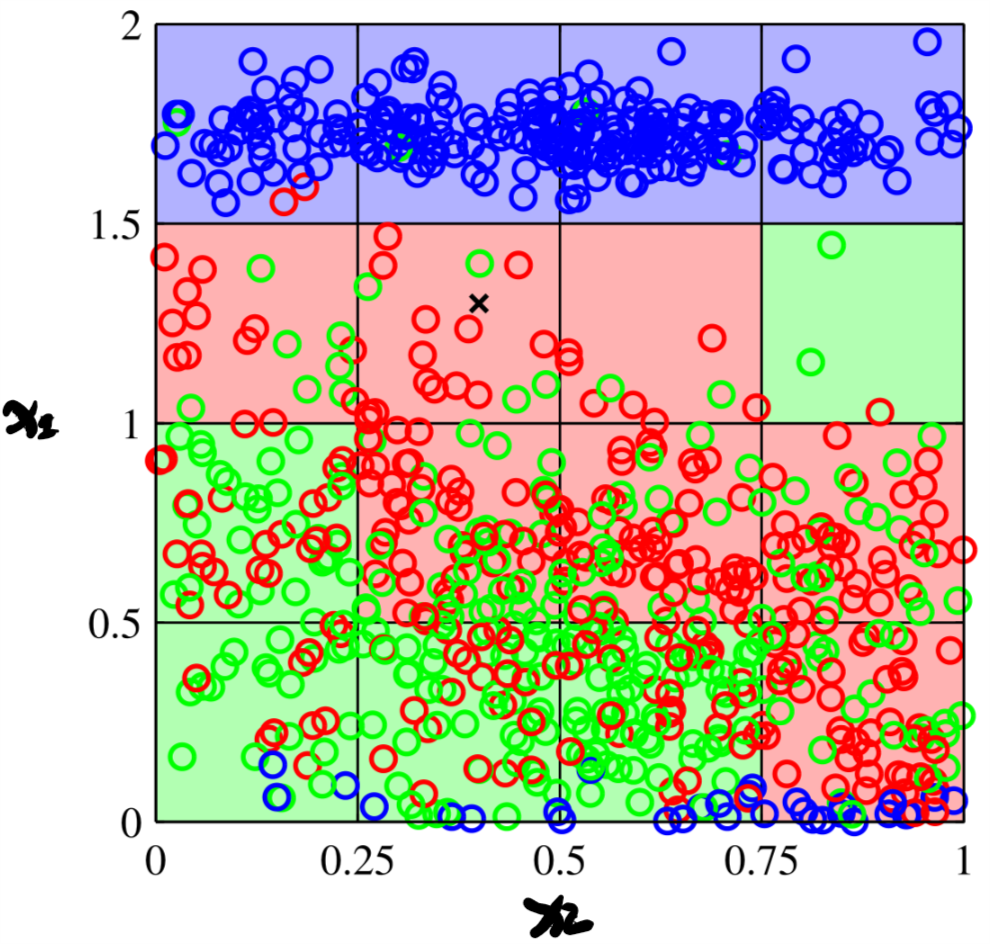
\includegraphics[width=0.6\textwidth]{../../img/computer_prml/20170503figure1dot20.png}
\caption{\label{fig:orgc0c41b0}
最近邻算法的简单实现}
\end{figure}


现在让我们再回到多项式拟合问题上来。假设输入是\(D\)维的而不是\(1\)维的。那么一个三阶的多项式拟合问题就变成:
\begin{equation}
\label{eq:1}
y(\mathbf{x}, \mathbf{w}) = w_{0} + \sum_{i=1}^{D}w_{i}x_{i} + \sum_{i=1}^{D}\sum_{j=1}^{D} w_{ij}x_{i}x_{j} + \sum_{i=1}^{D}\sum_{j=1}^{D}\sum_{k=1}^{D}w_{ijk}x_{i}x_{j}x_{k}
\end{equation}

式 (\ref{eq:1})的最高阶数是三阶,其需要估计的系数\(\mathbf{w}\)就到了\(D^{3}\)个。通常,为了更高的精度,我们需要更高阶的多项式,对于最高阶为\(M\)的多项式,其需要估计的系数是\(D^{M}\)个,呈指数增长。

\section{厚厚的西瓜皮}
\label{sec:org0060dab}


我们生活在一个三维世界中,所以让我们去想象四维空间的事情显得异常困难,但是数学上表示还是可以的。考虑一个\(D\)维空间的球,半径为\(1\),这个\(D\)维的球里嵌套了另一个\(D\)维的球,半径为\(1-\epsilon\)。问这两个球之间的体积占大球体积多大比例?

我们知道一个\(D\)维空间球半径为\(r\)的球的体积可以表示为:
\begin{equation}
\label{eq:2}
V_{D}(r) = K_{D}r^{D}
\end{equation}
其中\(K_{D}\)是依赖于\(D\)的常数。那么前面问题的结论是:
\begin{equation}
\label{eq:3}
\frac{V_{D}(1) - V_{D}(1-\epsilon)}{V_{D}(1)} = 1- (1-\epsilon)^{D}
\end{equation}
为了对这个问题有更直观的感觉,我们画出了不同\(D\)关于\(\epsilon\)的函数。如图\ref{fig:orgd89db5a}所示。
\begin{figure}[htbp]
\centering
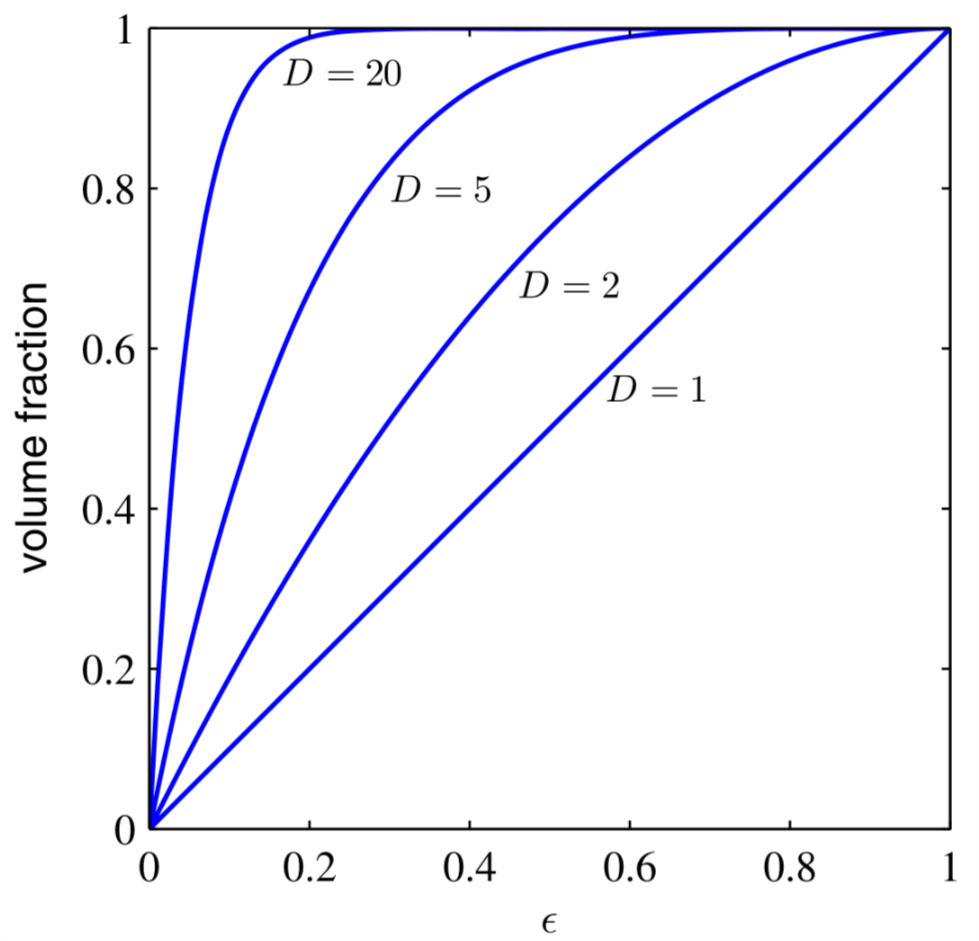
\includegraphics[width=0.6\textwidth]{../../img/computer_prml/20170503figure1dot22.png}
\caption{\label{fig:orgd89db5a}
两球之间的体积}
\end{figure}

从图\ref{fig:orgd89db5a} 我们可以看出对于固定的\(\epsilon\),随着维度的提升,两球之间的体积占大球的体积的比例越来越大。比如对于\(\epsilon = 0.1\),也就是说半径是\(0.9\)的\(D\)维空间中的球,当\(D\)是20 的时候两球之间的体积占了大球体积的85\% .也就是说如果在\(20\)维空间的这个球是西瓜的话,这个西瓜的西瓜皮就占了这个西瓜相当大的体积。

\section{高维空间的高斯分布}
\label{sec:org9483ee3}


现在我们考虑高维空间的高斯分布。在高维空间上,如果从笛卡尔空间转换到极坐标空间并且积分掉方向变量(也就是那个角度变量),我们就得到了一个与从零点出发的半径\(r\)有关的密度函数\(p(r)\)。那么\(p(r)\delta r\)就是在半径\(p(r)\)处薄薄的一层\(\delta r\)代表的概率。从图\ref{fig:orgd89db5a} 我们可以看到即使这薄薄的一层也占据了很大的概率空间。

\section{怎么办?}
\label{sec:org0353afe}


既然现实中很多问题都是高维,而在处理高维问题的时候,我们又碰到了维度诅咒。是不是就无计可施了呢?no!没有办法也要想办法,不然咋办呢?

事实上,尽管存在维度诅咒,在处理高维问题时,我们依然可以找到有效的解决方案。这基于两个事实:
\begin{enumerate}
\item 真实的数据通常只存在于输入空间的一个很小的子集。
\item 真实的数据通常展现一定的平滑特性,即对于输入的微小波动,输出也是仅仅是微小波动。所以我们可以通过插值的方法找到最优解。
\end{enumerate}

已有的模式识别算法都充分挖掘了这两个特性。
\end{document}
